
%%%%%%%%%%%%%%%%%%%%%% CHAPTER ONE %%%%%%%%%%%%%%%%%%%%%%%%%%%%%%%%%%%%%%%
\chapter{Installing Rocks}

\section{Rocks Installation}
We advise you to go through the rocks official \cite{rocksinstall} documentation  before the installation to understand the basic principles of clusters.\\
%Please refer to Appendix I for detailed steps.
\subsection{Physical Assembly}
The first thing to manage is the physical deployment of a cluster.The following diagram shows how the frontend and compute nodes must be connected:

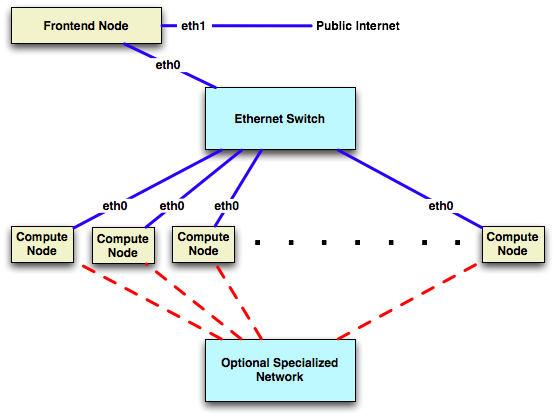
\includegraphics[scale=.5]{cluster.png} 
\paragraph{}
On the Compute nodes (Vm-container), the Ethernet interface that Linux maps to eth0 should be connected to the cluster's Ethernet switch. This network is considered private, i.e, all traffic on this network is physically separated from the external public network (e.g., The Internet).
On the Frontend, at least two Ethernet interfaces are required. The interface that Linux maps to eth0 should be connected to the same Ethernet network as the compute nodes. The interface that Linux maps to eth1 should be connected to the external network (Internet or your organization's intranet).
\paragraph{}
In our case the eth0 is connected to the switch placed within the rack and eth1 of the Frontend is connected to public network under Networks systems lab’s subnet.

\section{Frontend Installation}
The installation on the Frontend is done using a disk image either by a DVD or a bootable USB drive.The Jumbo DVD has all the required rolls in one single disk image. The x86 64 version of Rocks 6.1 can be downloaded from here \cite{rocksdownload}

\begin{itemize}
\item Insert the DVD/USB Drive and restart the main node (Frontend). A boot screen will be displayed with a prompt. Enter the following command to start the installation: 
 \item The next screen shows the list of all rolls in the DVD. Select the required rolls from the list. The Kernel, Base, OS and Web-Server rolls are mandatory. Additional rolls can be installed by using DVD based rolls. Hit next to proceed.
\item The next screen is for entering Cluster Information. Enter the details for Host name, cluster name, organization, locality, state, country, contact, URL, latitude and longitude. The fully-qualified host name is mandatory and is important for several cluster services.
 \item The next screen has the option to set the eth1 ( which is the interface to public network ) IP address. This is the public IP of the cluster(connected to the internet). Enter the public IP as 192.168.41.203.
 
\item The next screen has the option to set the private network eth0 IP address and netmask. This is the IP address of the private network between the Frontend and the nodes. The IP address used is 10.1.1.1 and the netmask is 255.255.0.0.

\item Now configure the gateway and DNS. Gateway used is 192.168.41.1 and DNS servers used are 192.168.254.2, 192.168.254.3.

\item Enter the root password of the cluster when prompted.
\item Configure the time by selecting the time zone for the cluster followed by inputting a Network Time Protocol(NTP) server that will keep the clock on the frontend in sync.

\item The next screen shows the option for the partitioning of the hard disk of the Frontend. Select "Manual Partitioning" since the configuration of " Auto Partitioning provides insufficient space for the /var partition which is used by the Eucalyptus Cloud to upload Virtual Machine Images.

\item The partition used for frontend is: \\ 
\end{itemize}

\begin{center}
\begin{tabular}{ | l | c | r |}
    \hline
    Partition Name & Size  \\ \hline
    /&170GB \\ 
    /var&480GB \\
	/export&170GB \\
	swap&1GB    \\
    \hline
  \end{tabular}
\end{center}


%%%%%%%%%%%%%%%%%%%%%% END OF CHAPTER ONE %%%%%%%%%%%%%%%%%%%%%%%%%%%%%%%%%%%%%%%
